\chapter{A Meta-Tool Architecture}
\label{kernelchapter}

\section{A Metamodelling Kernel}

The previous part of the book has shown how a rich metamodelling language such as XMOF allows the description of complex languages.  XMOF is a language and like any other language has a semantics.  If its semantics are not well understood then the rigour of any language defined using XMOF is compromised.  Up until now, questions of XMOF's semantic soundness have been avoided, instead informal descriptions of the constructs have been given.  This part of the book examines the semantics basis of XMOF in more detail and demonstrates how its semantics can be described in terms of the kernel language core-XMOF (a subset of XMOF itself).

% Even if the semantics of XMOF are described in terms of some other language, an obvious (recursive) question is - what should that language be defined in terms of?  Often the ultimate language is mathematics because of its universally consistent interpretation.  But mathematical descriptions of even simple languages can often be quite verbose and unpalatable to non-mathematicians.  Another option is to treat an implementation of a language as its semantic basis.  This approach is commonly used by programming languages such as Java and C++.  If a programmer wishes to understand the semantics of a particular program language construct, a program can be written which uses the construct and the resulting behaviour observed.

%In this chapter the former approach is taken.  However, rather than using mathematics the preference is to make core-XMOF so simple that the semantics can be understood from informal descriptions.  Using the informal descriptions of core-XMOF it is a short step to creating a programming-language-like machine which can interpret the kernel.  This would effectively be a virtual machine for XMOF.

\section{The Language Tower}

The first part of the book demonstrates how metamodels can be built using XMOF as a base language.  By virtue of being a language, XMOF must be an instance of some other language, that language is core-XMOF.  This kind of architecture gives rise to the language tower an example of which is illustrated in figure \ref{tower} (a).

There are two related issues with the tower of \ref{tower} (a).  Firstly the need to define XMOF in terms of a further language begs the question, what language should that further language be defined using?  This question is recursive because languages can be continually inserted at the foundation of the tower without ever bottoming out.  The second issue is that there are several different types of layers within the example tower of figure \ref{tower} (a):

\begin{figure}[htb]
\begin{center}
\subfigure[An illustration of a language tower]{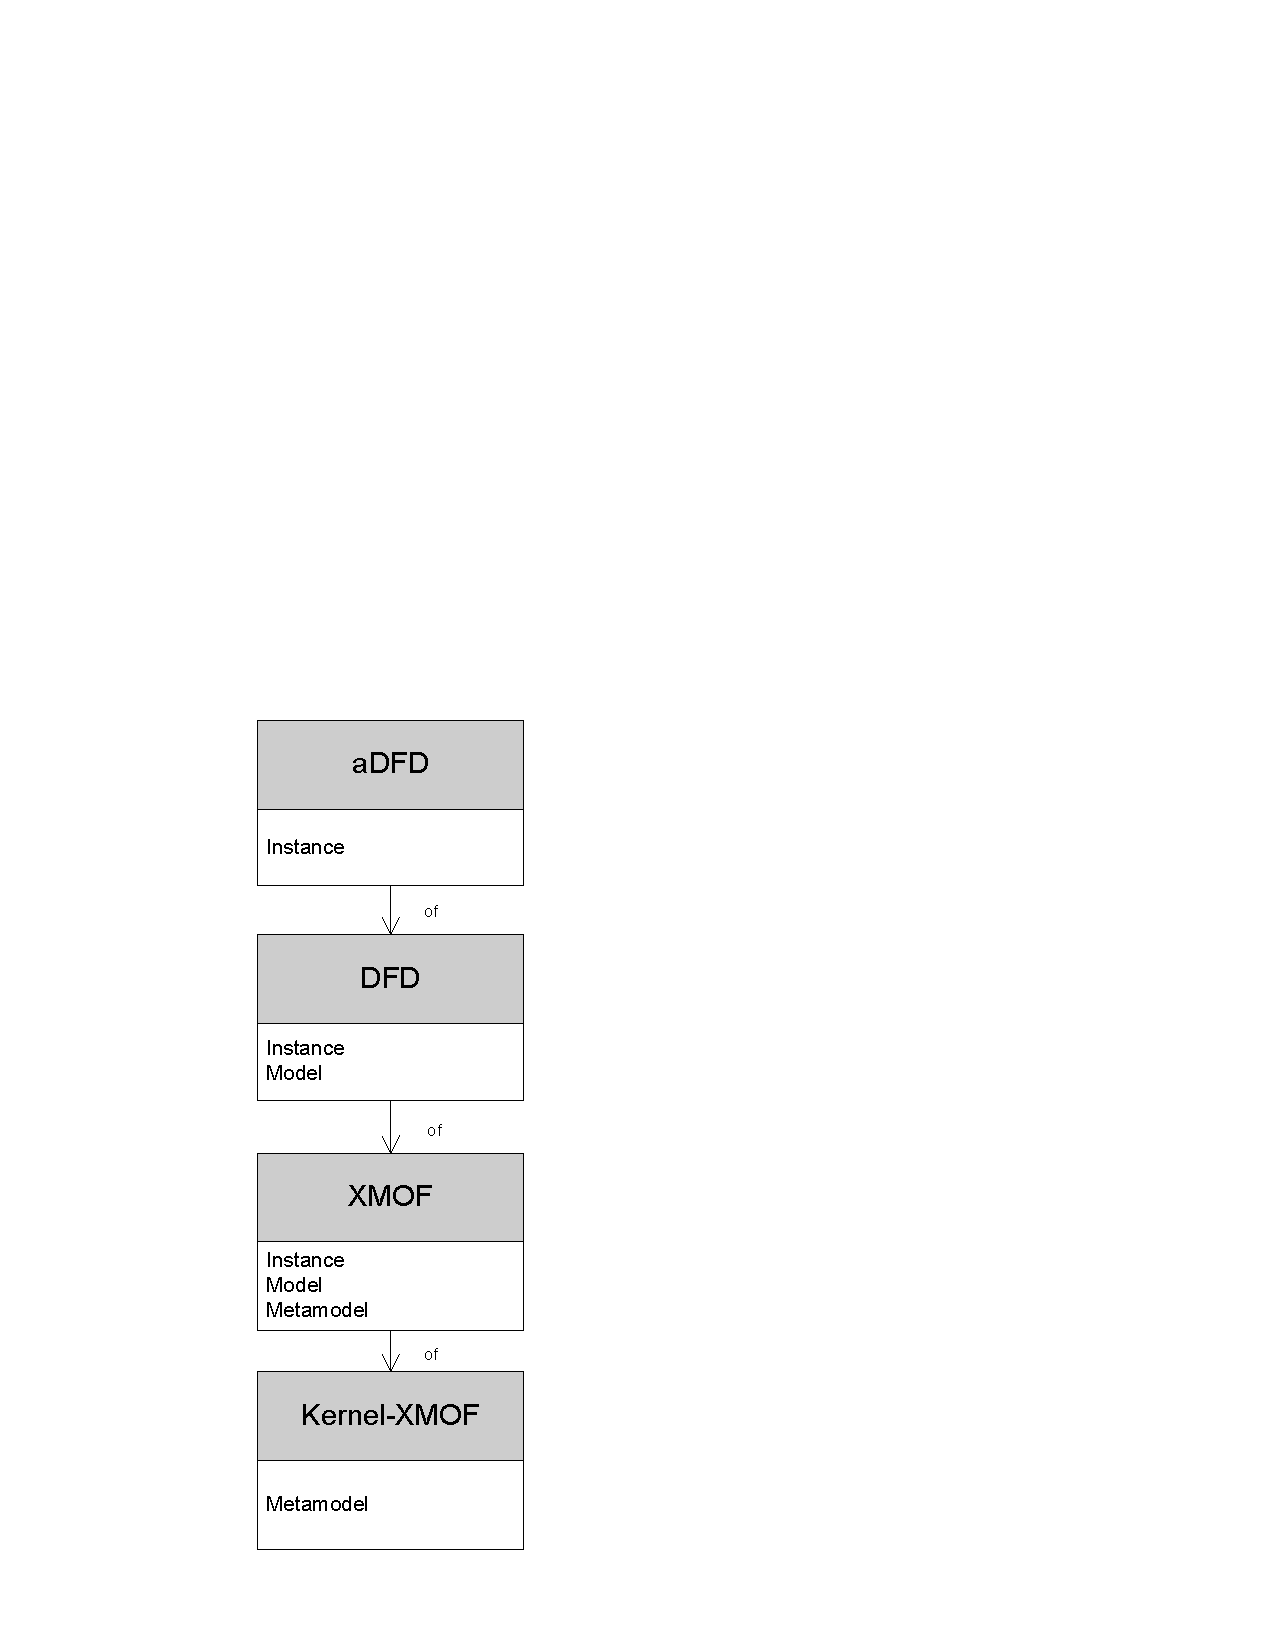
\includegraphics[width=4cm]{MetaToolArchitecture/figures/tower1.pdf}}
\subfigure[Introducing uniformity into the tower by making the bottom layer self defining]{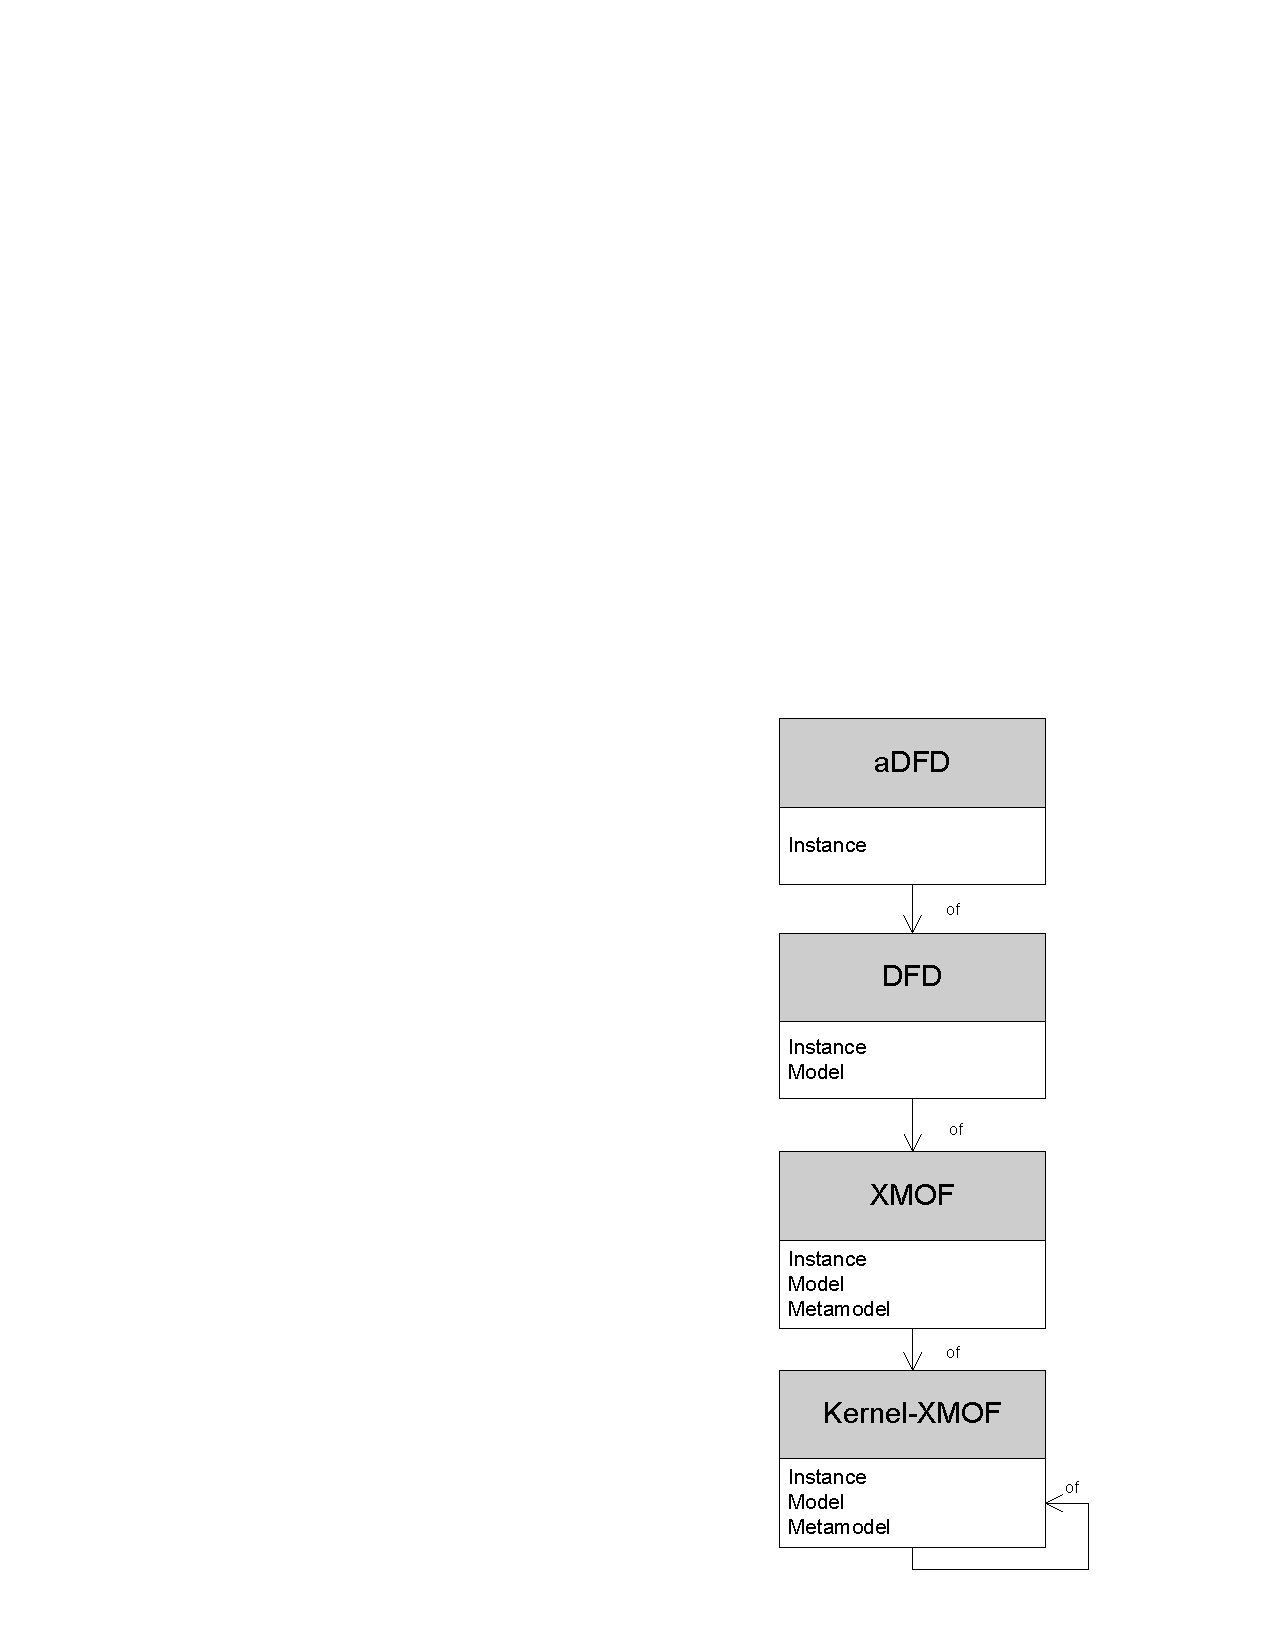
\includegraphics[width=3.8cm]{MetaToolArchitecture/figures/tower2.pdf}}
\caption{Language towers}
\label{tower}
\end{center}
\end{figure}

\begin{itemize}
\item Layers which are model instances (aDFD).
\item Layers which are instances and are models for instances (DFD).
\item Layers which are instance, models and metamodels for instances (XMOF).
\item Layers which are metamodels only (core-XMOF).
\end{itemize}

\noindent Although this may not seem problematic, the lack of uniformity in the architecture makes it complicated to define.  In a larger tower most layers would conform to that of XMOF in the sense that they would be an instance, model and metamodel.  As with the first issue, the problem rests with the base layer (core-XMOF) which is distinct from the other layers in that it is not an instance of any other language.

A solution to this problem is described in \cite{objVlisp} and involves making the base layer self defining as illustrated in figure \ref{tower} (b).  This solves the first issue mentioned because every layer is now an instance.  The self dependency also provides a much greater level of uniformity because there are fewer types of layers to consider:

\pagebreak
\begin{itemize}
\item Every layer is an instance;
\item a layer can be a model for instances;
\item or, a layer can be a model and metamodel for instances;
\end{itemize}

The architecture exemplified in figure \ref{tower} (b) is used as a basis for core-XMOF which will be described in the remainder of this chapter.  Despite the self defining nature of core-XMOF, it is important to recognise that an external language is still required to define core-XMOF.  The self defining nature creates a closed world for creating languages, this world is elegant because it requires few semantically distinct concepts in order to realise it.  Because there are fewer concepts, this also reduces the dependency on the world outside of core-XMOF, but that world must still exist.  This effectively gives rise to a towers-within-towers architecture an example of which is illustrated in figure \ref{towerOfTower} where the core-XMOF tower is defined using C++.  It is interesting to note that all concepts within a tower can be viewed as instances of the containing tower.  In the case of figure \ref{towerOfTower} the core-XMOF based languages can be viewed as an instances of C++.

Programming languages are a good way of defining core-XMOF because the result is a machine that will interpret languages constructed from core-XMOF and the imperative aspects of core-XMOF will execute.  From the point of view of comprehending the semantics of a language, this is advantageous because the semantics of a particular construct can be understood by executing an instance of that construct.  For the purpose of presenting semantics on paper it is less than ideal because many mechanisms must be introduced which are superfluous to the essence of the semantics, these are there to \emph{make the implementation work} in a particular programming language.

An alternative approach is to ground the kernel in a non executable language which has a universal consistent interpretation such as maths.  But mathematical descriptions of even simple languages tend to be quite verbose and unpalatable to non-mathematicians.  For this reason, this chapter resorts to explaining core-XMOF informally.  Although informality is never ideal, it is perhaps more appropriate in the case of core-XMOF because, as has been previously explained, core-XMOF has few distinct concepts.  Using the informal descriptions it is a short step to creating a core-XMOF programming-language-like machine which can interpret the kernel.  Details of how to implement interpreters for similar languages in Java can be found in \cite{programLanguageProcessors}.


\begin{figure}[htb]
\begin{center}
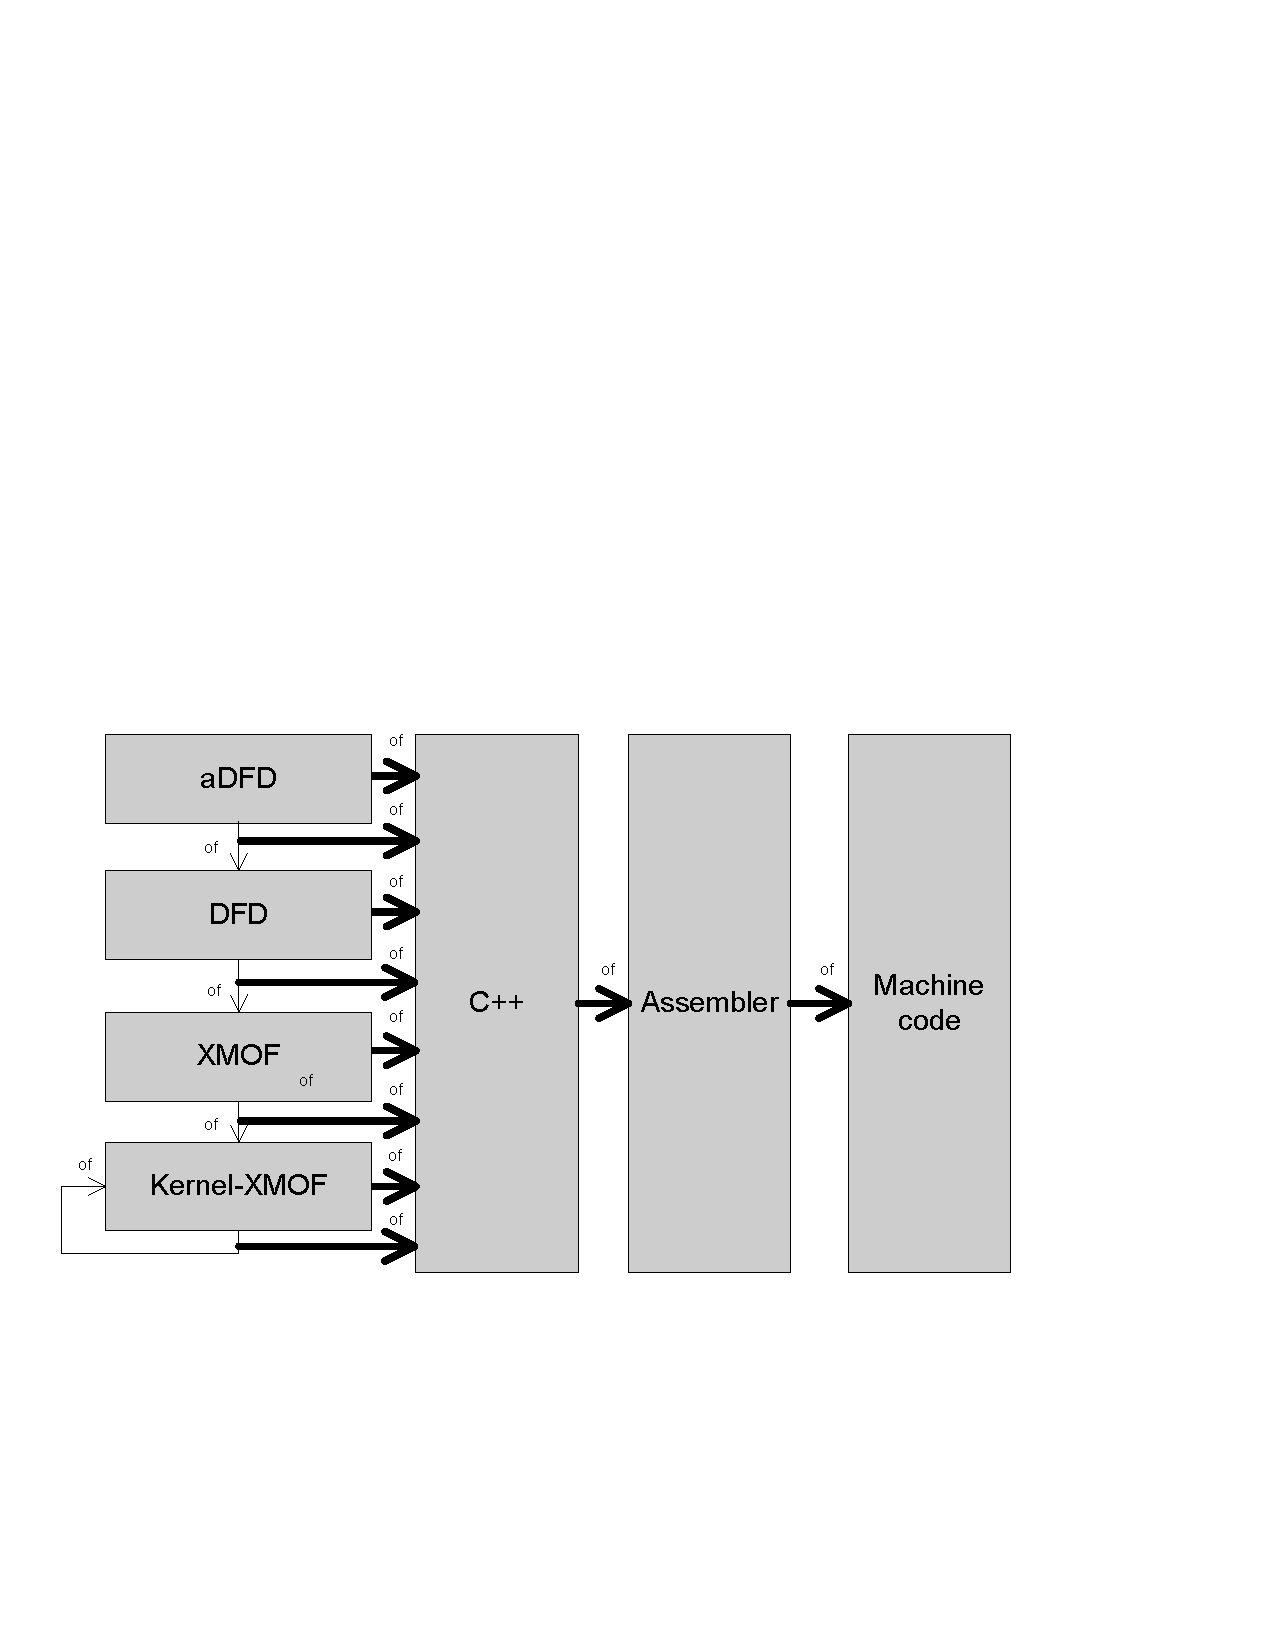
\includegraphics[width=12cm]{MetaToolArchitecture/figures/towerOfTower.pdf}
\caption{A language tower containing another language tower}
\label{towerOfTower}
\end{center}
\end{figure}

\section{Building the Tower}

Having simplified the language tower framework, it is now necessary to understand how to build such a tower.  To recap the requirements for the tower are: every layer is an instance, a layer can be model for instances or, can be a model and metamodel for instances.  One object oriented approach that provides a concise framework for addressing these requirements can be found in \cite{objVlisp}.  In this there are two class:

\begin{itemize}
\item Class: defines a model for instances which are the basis for further instances (a metamodel).
\item Object: defines a model for instances (a model).
\end{itemize}

\noindent Using these classes in two different configuration enables the requirements listed above to be dealt with.  An example of the first configuration is illustrated in figure \ref{core2}.  In this \emph{Animal} is a model because it is an instance of \emph{Class}, and is an instance itself because \emph{Class} inherits from \emph{Object}.  \emph{Chicken} and \emph{Dog} are instances because \emph{Animal} inherits from \emph{Object}.

\begin{figure}[htb]
\begin{center}
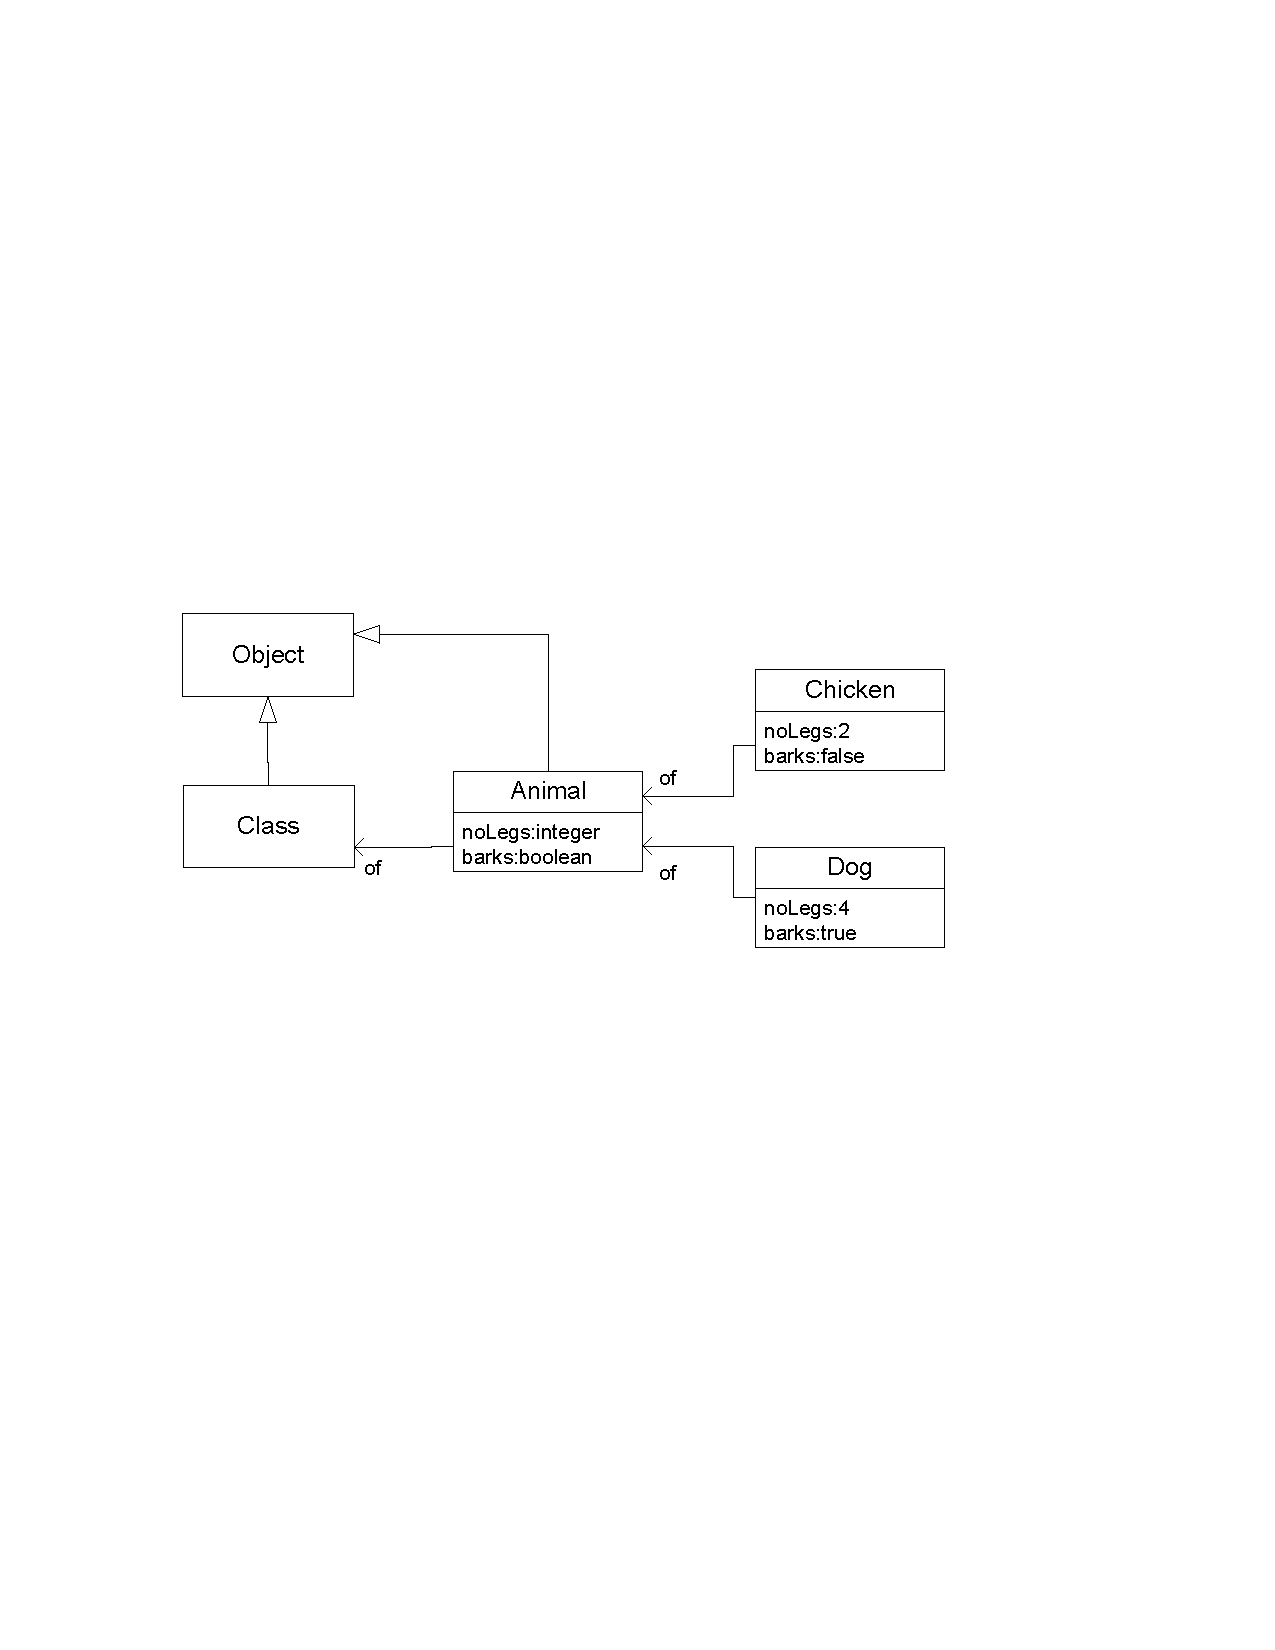
\includegraphics[width=9cm]{MetaToolArchitecture/figures/core2.pdf}
\caption{Defining instances who instances are terminal (models)}
\label{core2}
\end{center}
\end{figure}

An example of the second configuration is shown in figure \ref{core3}.  Here \emph{Statemachine} is the basis for further instance because it is an instance of \emph{Class}, and is an instance itself because \emph{Class} inherits from \emph{Object}.  Because \emph{Statemachine} inherits from \emph{Class} then instances of \emph{Statemachine} can also be the basis for further instances.  \emph{Statemachine} is an object because it is an instance of \emph{Class} which inherits from \emph{Object}.  \emph{Switch} is an object because it is an instance of \emph{Statemachine} which inherits from \emph{Object}, and \emph{Switch1} and \emph{Switch2} are objects because they are an instance of \emph{Switch} which inherits from \emph{Object}.

\begin{figure}[htb]
\begin{center}
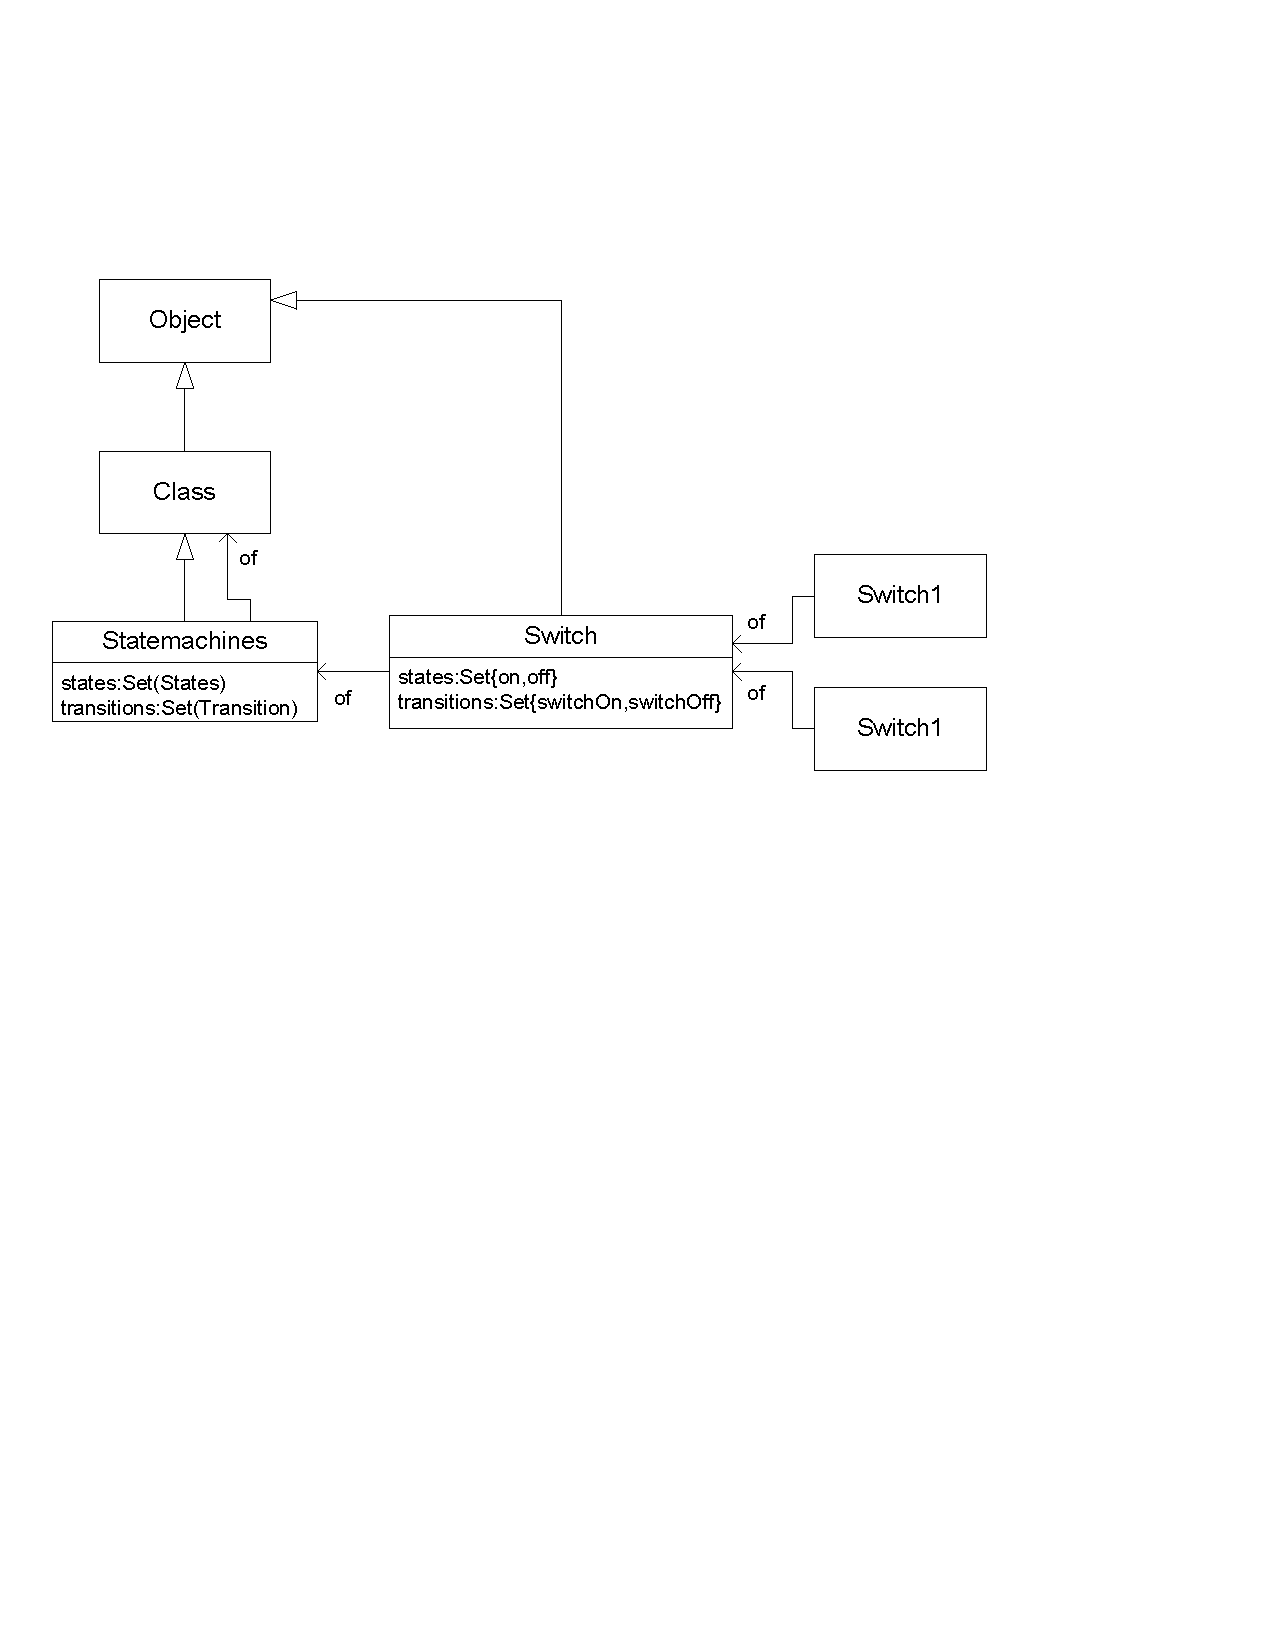
\includegraphics[width=10cm]{MetaToolArchitecture/figures/core3.pdf}
\caption{Defining instance who instances can have instances (metamodels)}
\label{core3}
\end{center}
\end{figure}

Figures \ref{core2} and \ref{core3} are not however an accurate representation of the self defining language tower since the bottom layer \emph{Class} is not an instance of itself.  This is rectified by introducing the configuration illustrated in figure \ref{core1}, this configuration is often referred to as the \emph{golden braid} \cite{geb} because of the mutual dependencies between its components.  The self defining base level is described by \emph{Class} being an instance of itself.  Note that \emph{Class} is also an object because of it is an instance of \emph{Class} which inherits from \emph{Object}.

\begin{figure}[htb]
\begin{center}
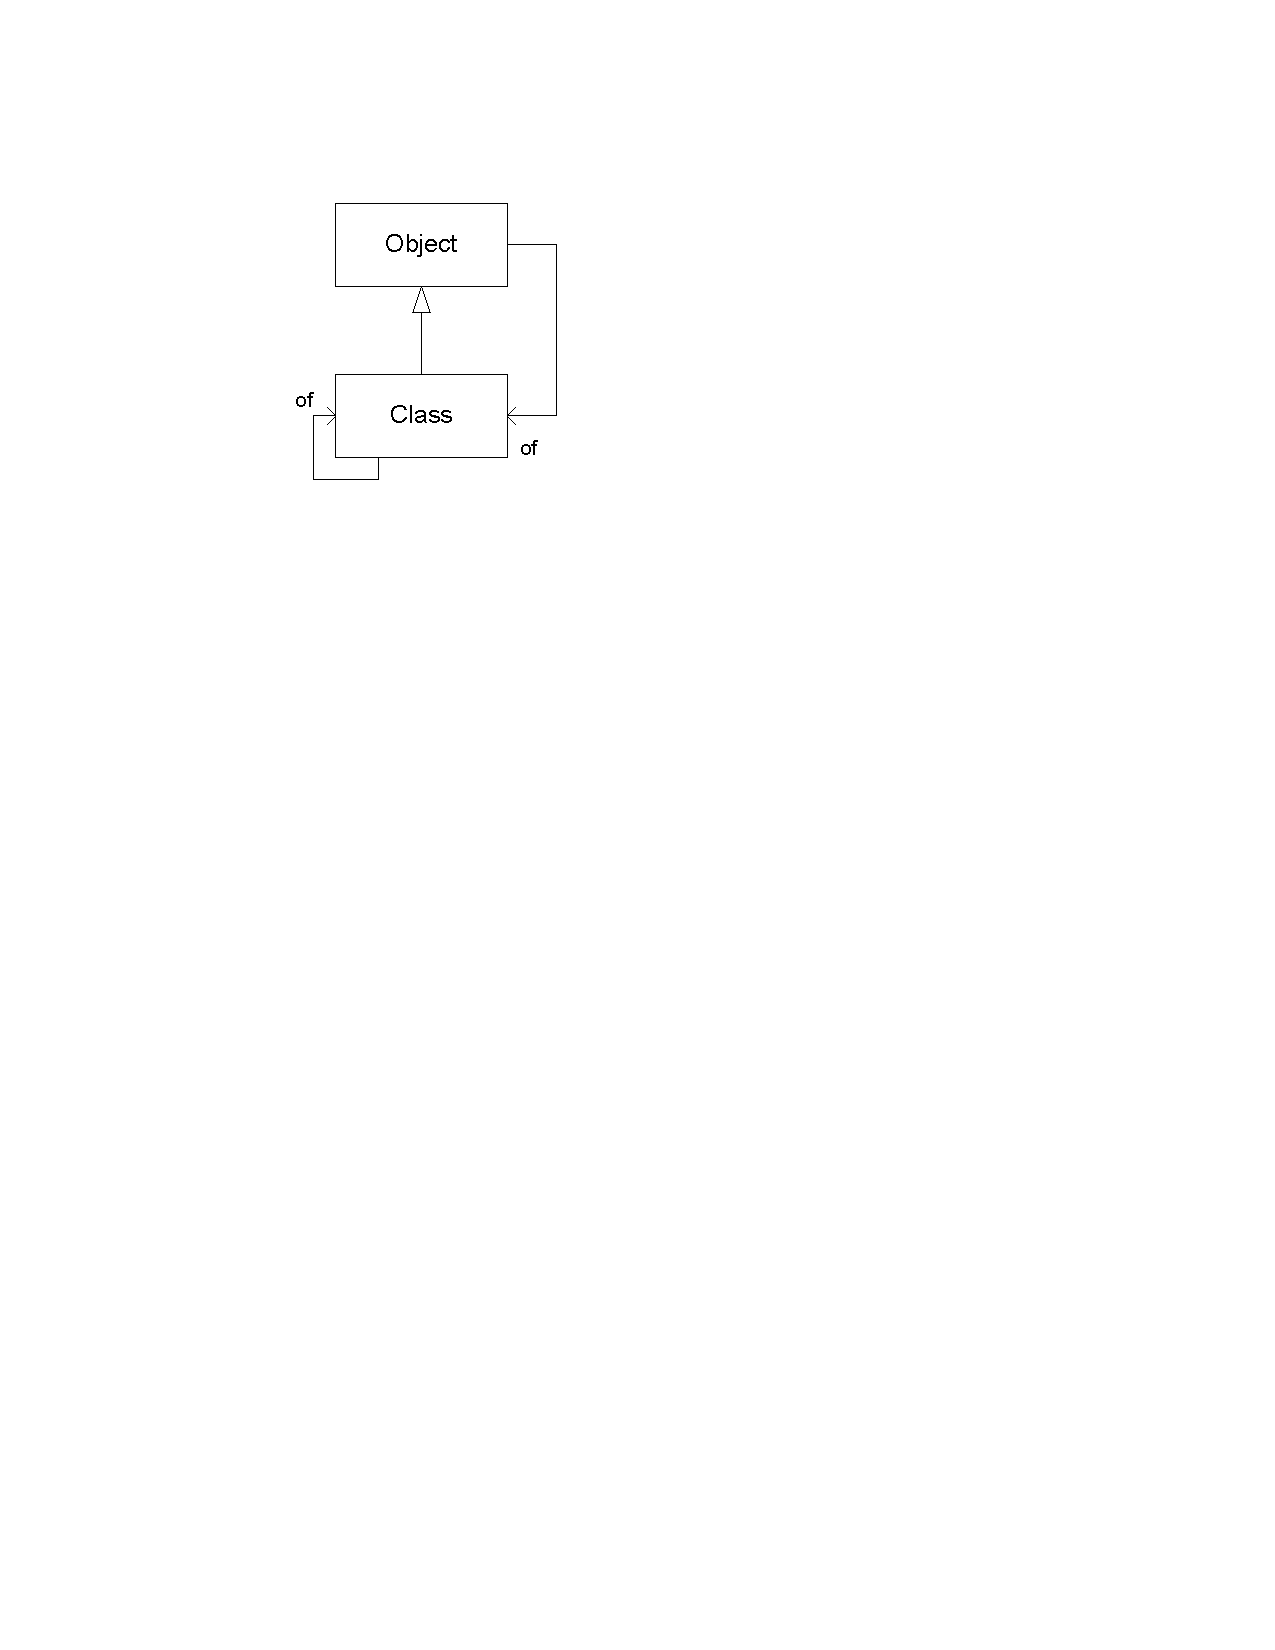
\includegraphics[width=3cm]{MetaToolArchitecture/figures/core1.pdf}
\caption{The self defining configuration}
\label{core1}
\end{center}
\end{figure}

The configuration of \ref{core1} forms the heart of core-XMOF and enables core-XMOF to be used to build language towers.  Although these configuration may seem confusing at first, they are an elegant approach to language architecting because there are few primitive concepts to understand the semantics of (these are effectively instantiation and generalisation).  The semantics of these could be given in some mathematical language, or implemented in a programming language.  As mentioned in the introduction the preference is to treat these concepts as the fundamental language and explain them informally without need for an external system.  In the next section we describe the semantics of core-XMOF in more detail.

\FloatBarrier

\section{Core-XMOF}

In this section the core-XMOF kernel is introduced in more detail. This involves putting `meat on the bones' of the configurations described in the previous section and more concretely describing the mechanics of the kernel.

\begin{figure}[htb]
\begin{center}
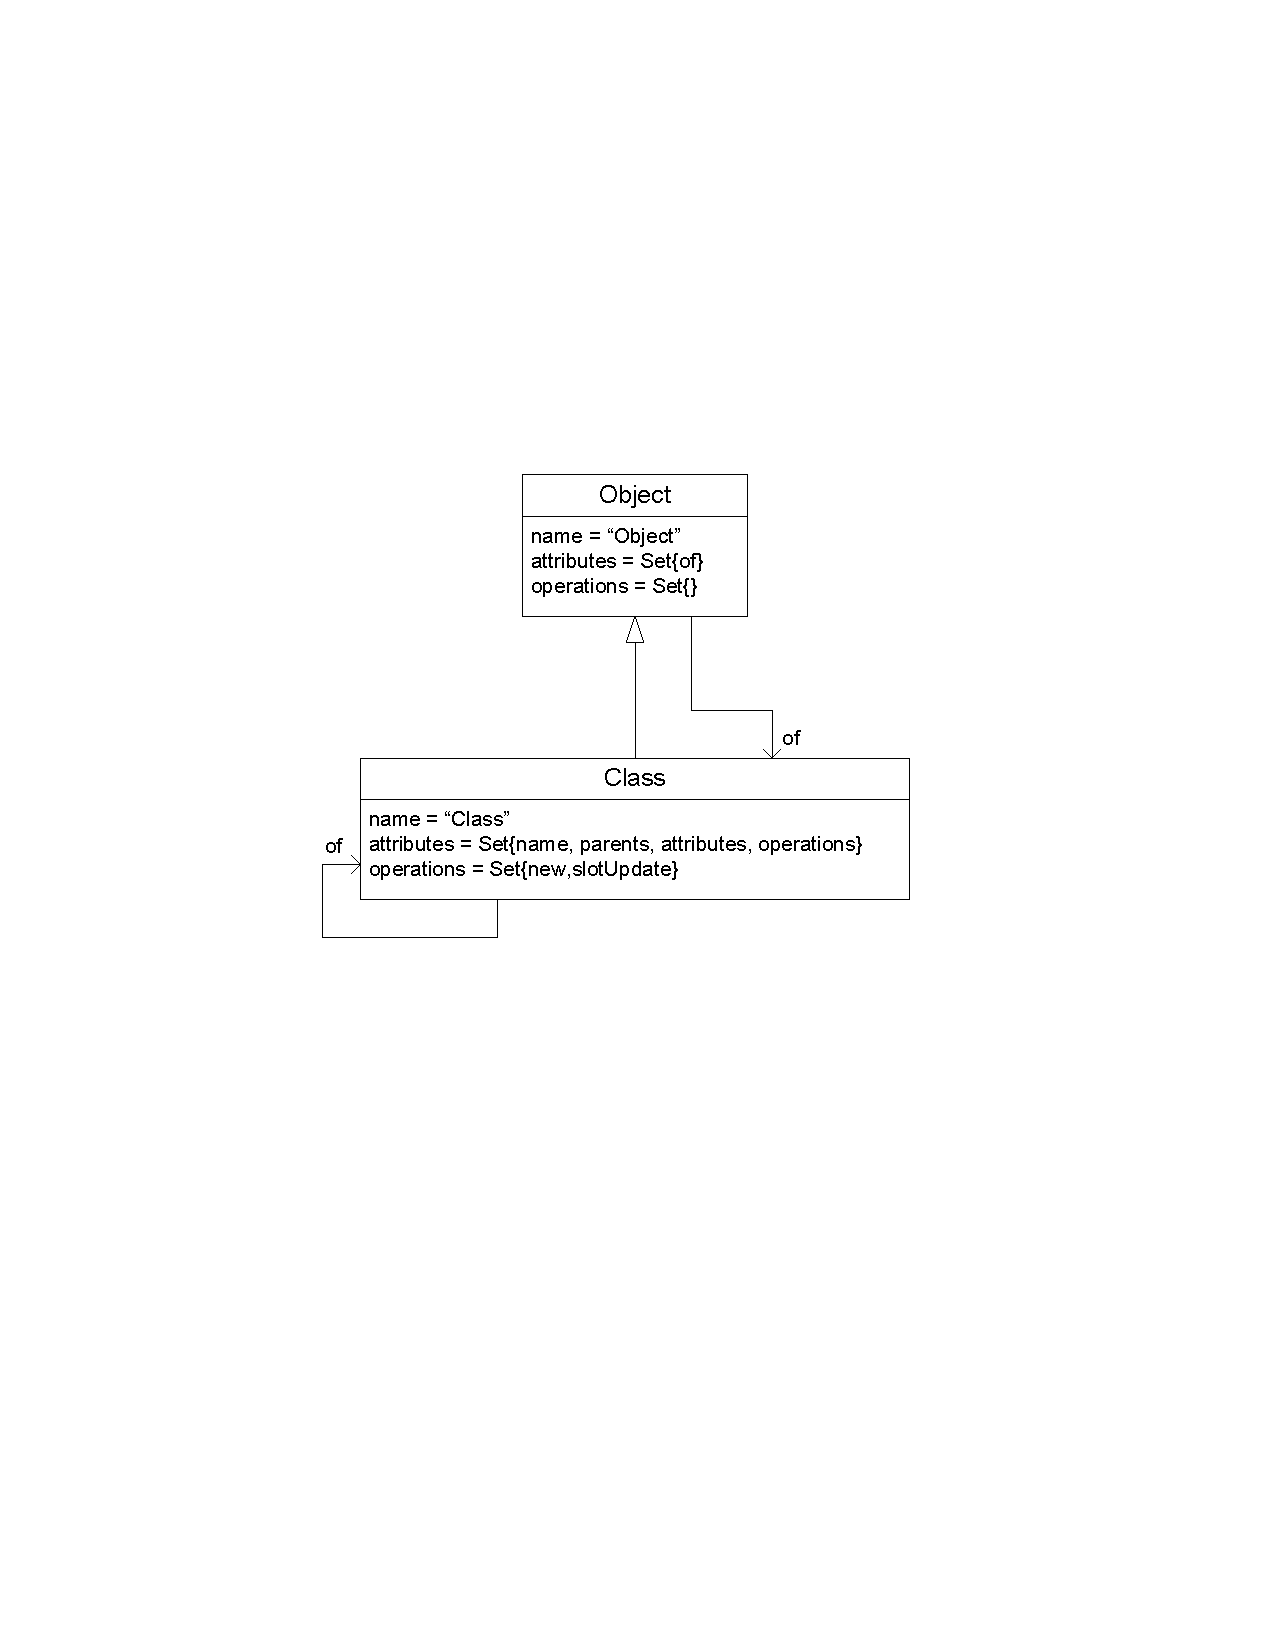
\includegraphics[width=8cm]{MetaToolArchitecture/figures/moreDetail.pdf}
\caption{The self defining configuration in more detail}
\label{moreDetail}
\end{center}
\end{figure}

Figure \ref{moreDetail} illustrates the Class/Object configuration once again but this time augmented to include their slots.  Class has four slots \emph{name}, \emph{parents}, \emph{attributes}, \emph{operations} and \emph{of} (\emph{parents} is depicted diagrammatically by the inheritance arrow).  The slots of an object correspond directly to the attributes of the object's class.  In the case of Class, its slots are the union of the attributes of Class and Object (because of the inheritance relationship).  The direct correspondence between a Class's attributes and slots is what makes Class self defining.

When an operation is invoked on an object, the operation lookup protocol navigates to the object's class in order to find the appropriate operation.  The means by which objects are instantiated is specified by the \emph{new} operation in Class, this operation is special because it is one of two operations whose semantics are specified outside of the kernel.  The semantics of \emph{new} have been hinted at already and involve a number of steps:

\begin{itemize}
\item Calculating the union of the class's attributes and the attribute's of the class's parents.
\item Creating a new object with slots corresponding to each of the class's attributes.
\item Setting the value of the \emph{of} slot to that of the class responsible for the instantiation.
\end{itemize}

\noindent A further example of this is shown in figure \ref{moreDetailExample2} where the class \emph{Animal} has a set of attributes defining \emph{name}, \emph{noLegs} and \emph{barks}.  The resulting object has slots for each of these attributes plus \emph{of} since \emph{Animal} inherits from \emph{Object}.

% Operations performed on the class

\begin{figure}
\begin{center}
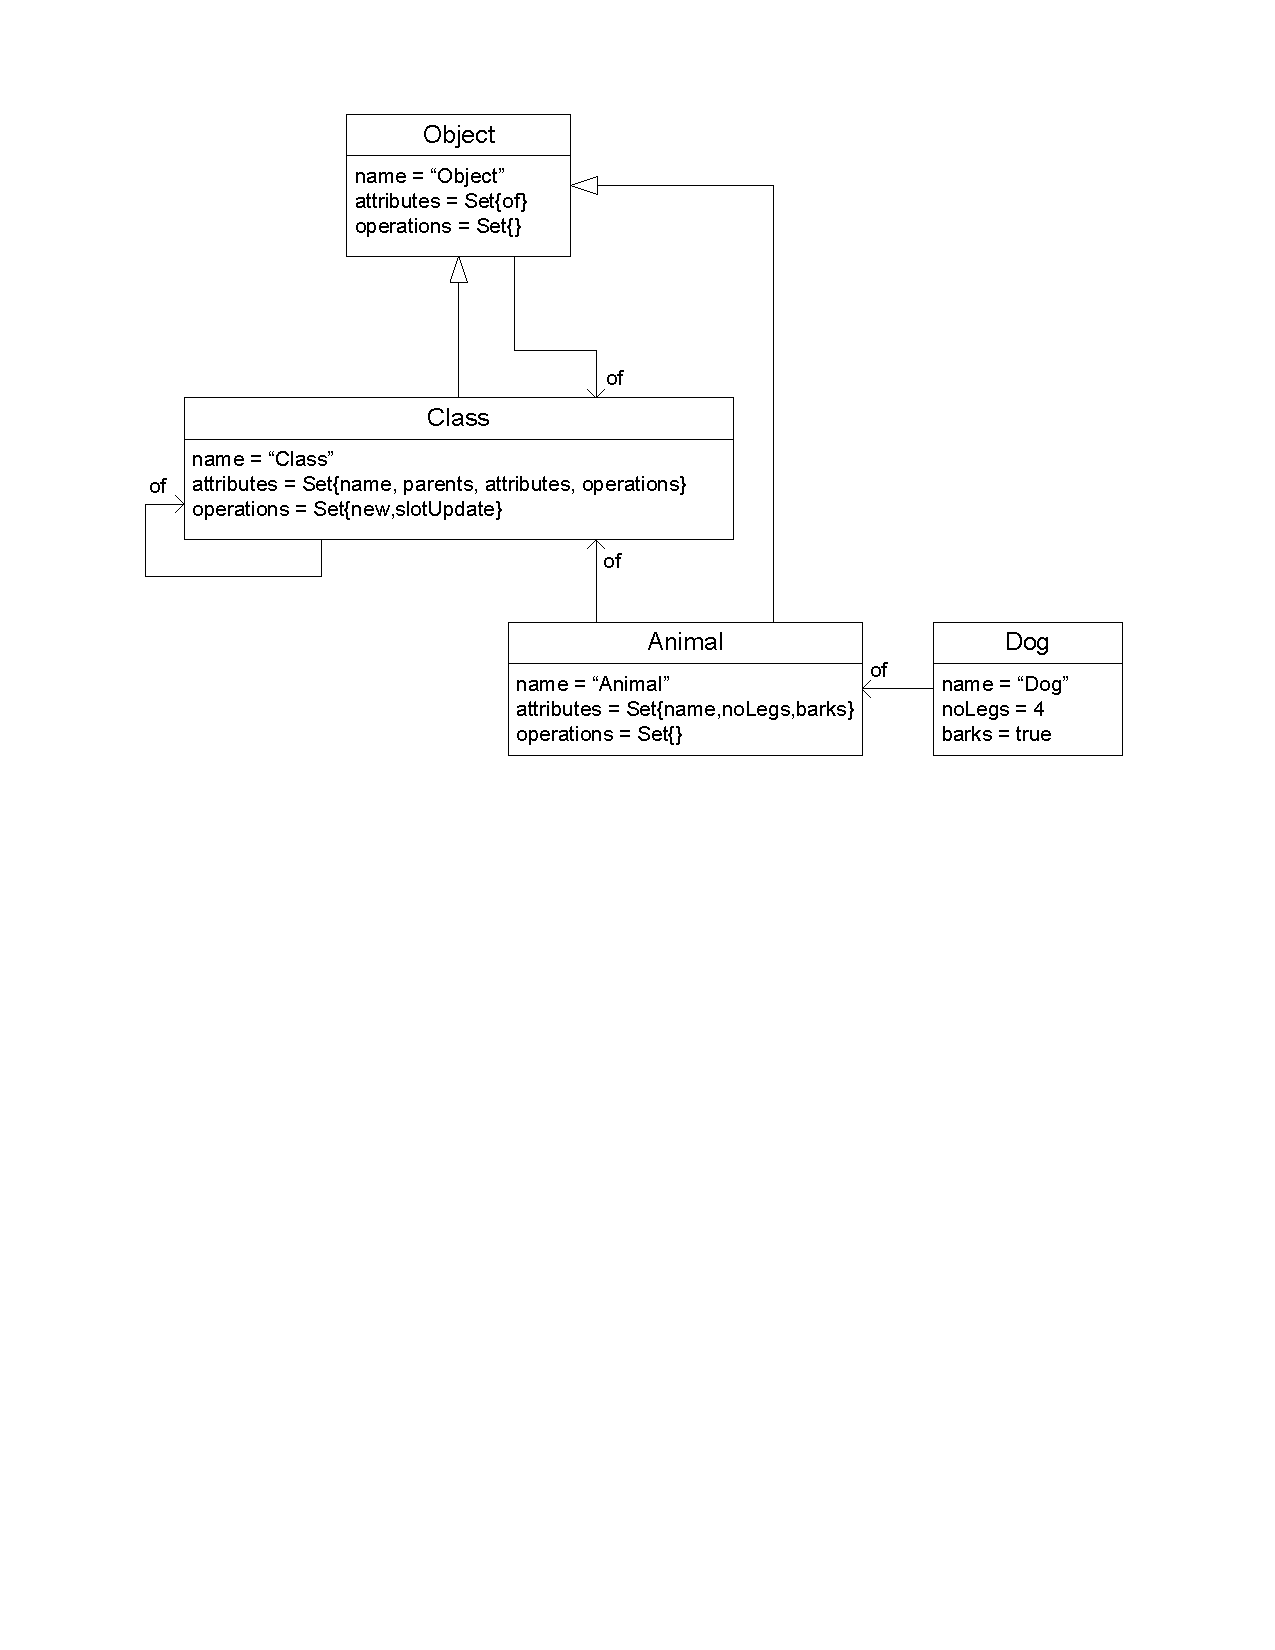
\includegraphics[width=12cm]{MetaToolArchitecture/figures/moreDetailExample2.pdf}
\caption{An illustration how of how a class's attributes defines the slots of its objects}
\label{moreDetailExample2}
\end{center}
\end{figure}

\begin{figure}
\begin{center}
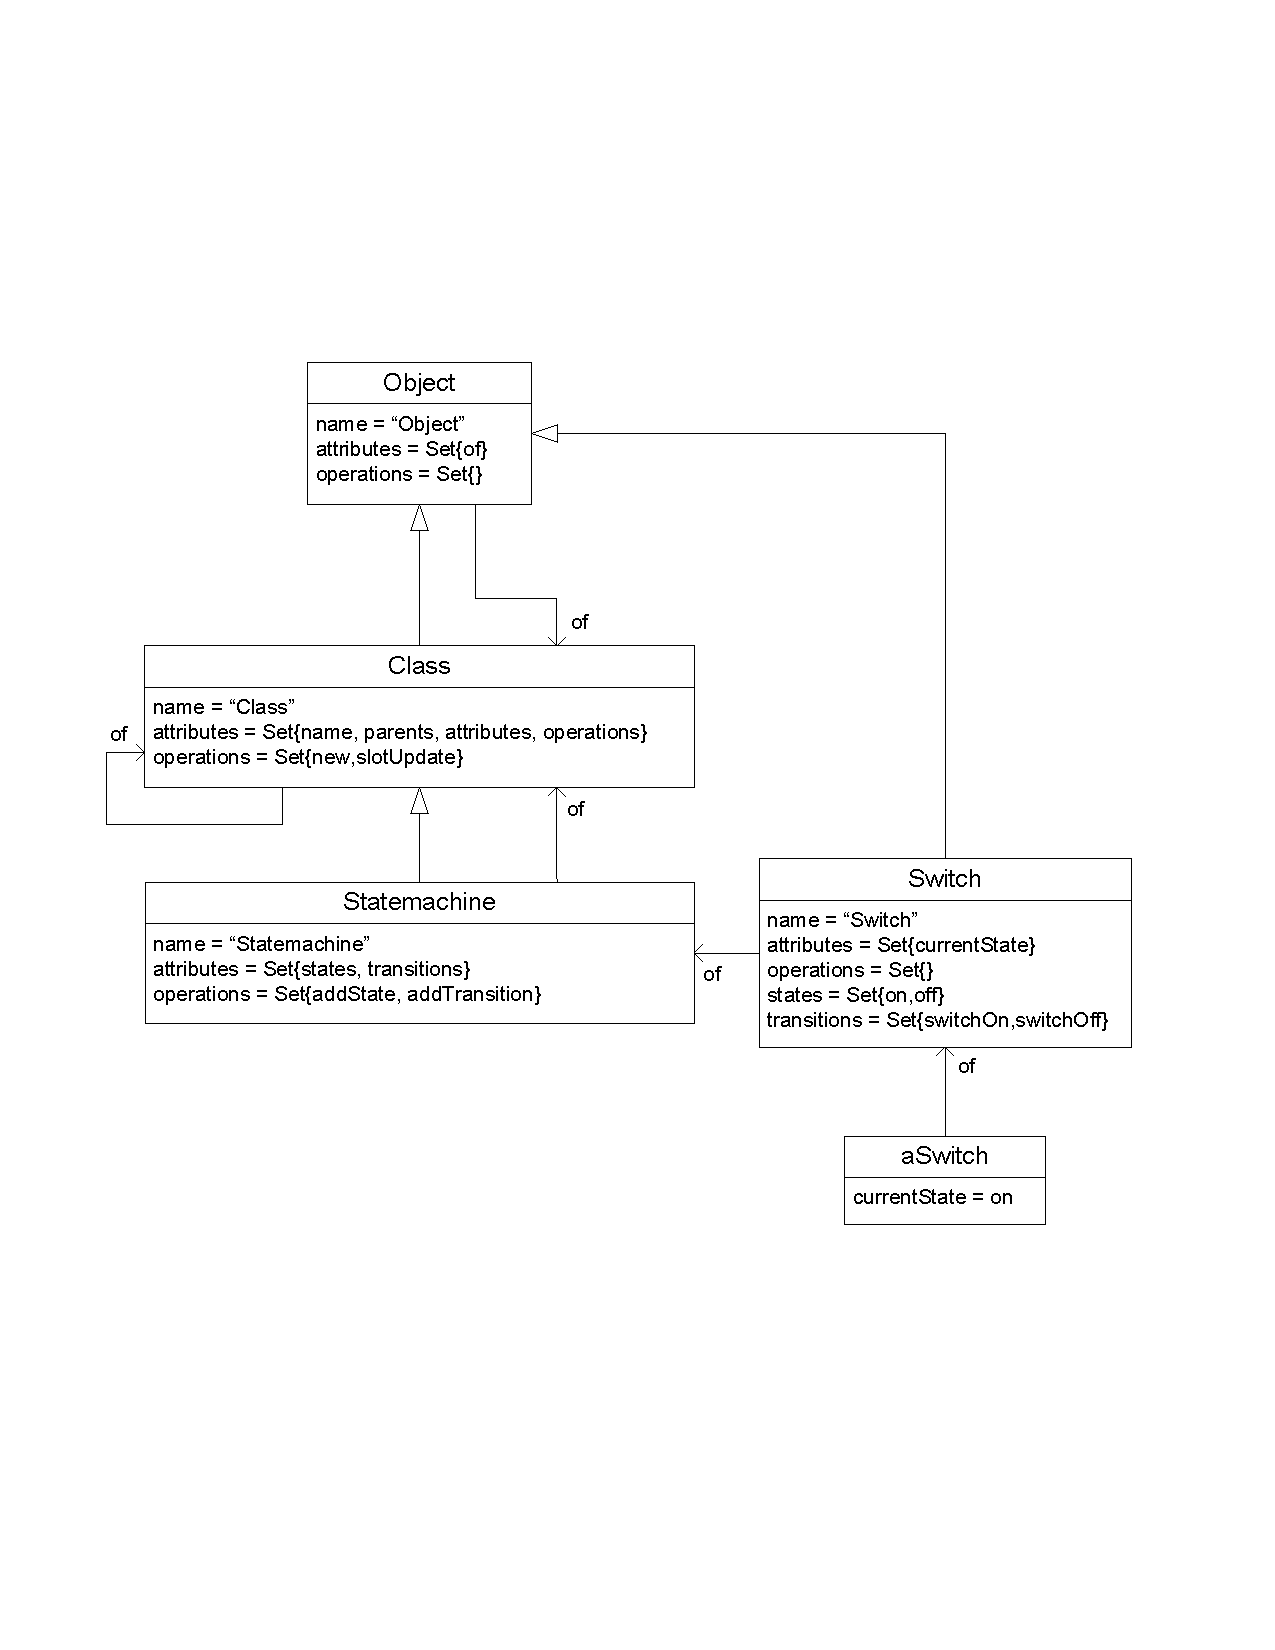
\includegraphics[width=12cm]{MetaToolArchitecture/figures/moreDetailExample.pdf}
\caption{The self defining configuration}
\label{moreDetailExample}
\end{center}
\end{figure}

\section{Class Diagrams}

Having defined the foundation kernel-XMOF in the previous sections, this section demonstrates how the metamodel for class diagrams can be constructed using the kernel.

\section{OCL and OCL++}

The earlier part of the book demonstrates how OCL and OCL++ are key components in a language engineers armoury.  In this section it is shown how these languages can be metamodelled using the core-XMOF kernel.

\section{Mappings}

If the relationships between metamodels cannot be understood, then the ability to use multiple models to describe systems is of limited use.  Chapter \ref{} illustrates how a mapping can be constructed between two diverse metamodels.  This section grounds the semantics of that mapping language using kernel-XMOF.

\section{Conclusion}
